\newpage

\section{Durchführung}
\label{sec:Durchfuehrung}
Zur Messung wird eine $2\,\unit{\mega\hertz}$-Sonde verwendet. Die Messwerte werden mit dem Programm EchoView
dargestellt. Als Kontaktmittel wird bidestilliertes Wasser verwendet. Über ein Steuergerät lässt sich einstellen,
ob das Durchschallungs- oder Impuls-Echo-Verfahren verwand werden soll. Weiterhin lässt sich ein
Verstärkungssignal hinzuschalten, dass die Sichtbarkeit von kleinen Amplituden gewährleistet.\\
Zu Beginn werden mit einer Schieblehre die Maße der zu vermessenden Acrylzylinder bestimmt. \\
Danach wird mit dem Impuls-Echo-Verfahren die Laufzeit des Echos für fünf unterschiedliche Konfigurationen bestimmt. Um die
Zylinder aufeinander zu stellen wird das Kontaktmittel verwendet. Gleiches wird mit dem Durchschallungsverfahren
noch einmal gemessen und anschließend überprüft. \\
Weiterhin wird mit dem Impuls-Echo-Verfahren die
Amplituden der eingehenden und reflektierten Welle für die fünf Zylinderkonfigurationen gemessen und daraus die
Dämpfung bestimmt. \\
Abschließend wird mit Hilfe des Impuls-Echo-Verfahrens die Abmessungen eines Augenmodells
bestimmt. Dazu wird mit leichtem Druck der Einfallswinkel so verändert, dass ein Echo an der Retina erkennbar
wird.\\
In \autoref{fig:auge} ist eine schematische Darstellung des Modellauges zu finden. Die
Schallgeschwindigkeit der Linse ist mit $c_{\symup{L}} = 2.500\,\unit{\meter\per\second}$ und die der
Glaskörperfüssigkeit mit $c_{\symup{GK}} = 1.410\,\unit{\meter\per\second}$ gegeben \cite{sample}.

\begin{figure}
    \centering
    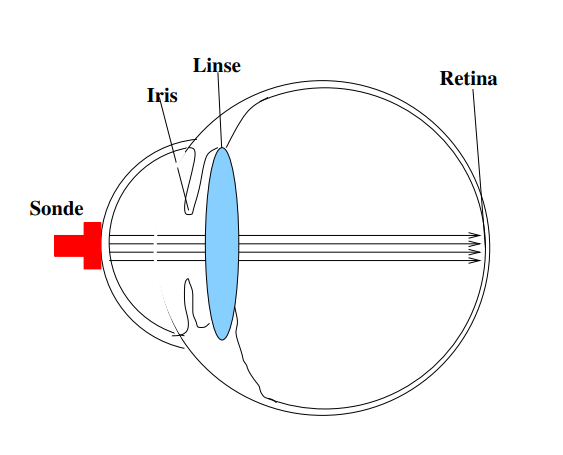
\includegraphics[width=0.5\textwidth]{messwerte/Versuchsaufbau.png}
    \caption{Schematische Darstellung des Augenmodells.}
    \label{fig:auge}
\end{figure}